\chapter{Theoretical Background}
This chapter will give a theoretical background for the technologies and techniques used in the subsequent chapters. It will provide a brief overview of the architecture and working principle of \acp{CNN}. Then, certain selected topics from 3D graphics are presented that give an understanding of principles that are used in this thesis. Lastly, this chapter will present fundamentals about game engines and robotics.

% //////////////////////////////////////////////////
\section{Convolutional Neural Networks}
Everyday tasks performed by humans require exact recognition and categorization of objects in order to perform actions like manipulating objects. 
% Beispiele, konkreter
These skills can further be used to deduce an understanding of one's surroundings and effectively grasp the context one acts in. These tasks are easily and for the most part subconsciously performed by humans but prove to be a challenge for software.\
\subsection{General Working Principle}
\acp{CNN} are a type of \acp{ANN} that operate on high-dimensional input data. This includes regular images in raster formats as their pixels are organized in rows and columns and color channels resulting in a three-dimensional input volume. These networks consist of multiple layers: the first layers will prepare the input data for later use (e.g. by performing scaling down the input data).\\
Next, \ac{conv} layers further process the input data. Those have a set of learn-able filters that are the artificial representation of biological neurons and perform convolutions on small chunks of data, that extend through the full depth of the input volume \cite{Schweitzer2017}, along the input data (e.g. by sliding through images row-by-row and column-by-column) where they process local pixel data depending on their implementation and the size of their receptive field. For instance, by performing edge-detection (using e.g. the Prewitt, Roberts or Sobel operators \cite{5557884}), filters may uncover features. Each of these filters will output a two-dimensional activation map that contains their responses at every position of the input data \cite{cs231n}. Stacking these activation maps yields a three-dimensional output volume.\\
The output of \ac{conv} layers is a linear function. In order to solve real-world problem that are non-linear though, non-linear layers are applied to the output of \ac{conv} layers. In simplified terms, those layers map the data from an input volume to a specified, non-linear range of values (e.g. from 0 to 1). There are various non-linear functions that can be used, a popular one is the \ac{ReLU} which maps negative values and keeps positive values. It is simple to implement and does not involve expensive computations.\\ %Drawbacks?
Pooling layers are used to reduce the size of the input data by applying filters to it. There are various methods that can be used, such as the average-pooling that chooses the average value of inputs. By reducing the size of inputs, pooling layers effectively reduce the complexity and number of weights in following layers, hence processing by following layers require less computation time. Chaining layers by using the output of one last layer as an input for another layer allows to detect more complex features as the filters of the other layers would be trained using refined data.\\
Lastly, at end of a \ac{CNN} will be one or more \ac{fc} layers. Those translate an input volume to a set of $n$ values where each value represents one class the network can choose. Each of these values would represent the probability of its class. This translation is done by learning from the input volume which is a stack of activation maps of complex features. Certain combinations of high values in those maps will indicate specific classes like the detection of a long body with multiple wheels on a flat ground may be interpreted as a vehicle.\\
Figure \ref{fig:lenet5} shows the architecture of LeNet5 by LeCun \textit{et al.} \cite{Lecun98gradient-basedlearning} from 1998. It should prove to set a pattern for modern \acp{CNN} by utilizing multiple sets of \ac{conv}, non-linearity and pooling layers, forwarding their processed data to multiple layers for classification. One of its successors is AlexNet, designed by Alex Krizhevsky \textit{et al.} in 2010 \cite{NIPS2012_4824} which is still a relevant measure for modern \ac{NN} today \cite{DBLP:journals/corr/CanzianiPC16}.

\begin{center}
\noindent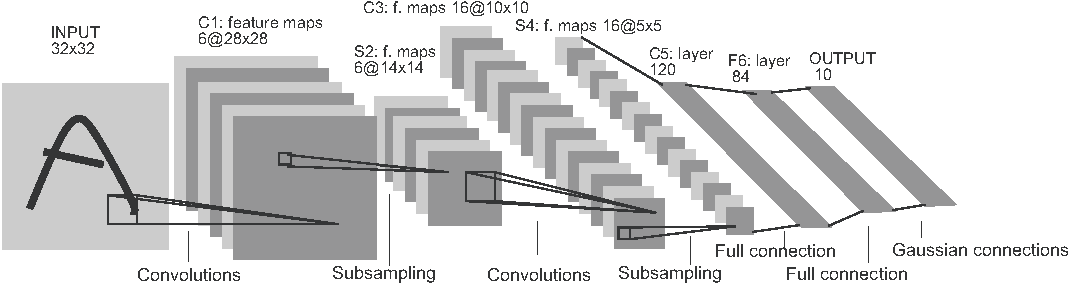
\includegraphics[width=12cm]{tex/img/ch03/LeNet5.pdf}
\captionof{figure}[Architecture of LeNet5]{Architecture of LeNet5 that set a pattern for modern \acp{CNN} \cite{Lecun98gradient-basedlearning}}
\label{fig:lenet5}
\end{center}

\subsection{Data Augmentation}
In summary it can be stated that \ac{conv} layers are trained to detect features and \ac{fc} layers are trained to detect relations between features that indicate specific classifiers. To achieve this, \acp{CNN} need to be trained with datasets specific to their application that must be of good quality \cite{Schweitzer2017}. Factors contributing to the quality of datasets are the quality of their images (e.g. high resolution, little noise) and labels (e.g. number of classes, general presence of regions associated with labels). However large sets of such data may be hard to come by due to scarce availability (e.g. of datasets for highly specialized applications) or the amount of effort creating those takes. Lastly, they may simple cost a lot of time to produce.\\
\emph{Data Augmentation} promises to solve this problem by altering datasets through application of various operations on them: for instance images can be stretched, mirrored, zoomed and rotated or color filters can be applied to them. As long as these changes are transferred to the labels of images, these altered datasets drastically increase the size of datasets that can be used for training \acp{CNN}. This can also potentially help to make detections more reliable for special cases: for instance, datasets that feature cars would mostly show cars in their surroundings, hence they would rarely be cut off in images. Altering images so they cut off parts of cars like wheels may enable \acp{CNN} to recognize cars without requiring cars to actually have wheels.
\clearpage

\section{Transforms}
\label{ch03-transforms}
In computer graphics, objects in 3D space are organized in a \emph{scene graph} where nodes use \emph{transforms} to express their location, rotation and scale relative to their parent node. Those attributes can be expressed in vectors with three elements each, where each of these elements represents the effect of a transformation for one axis. A complete transformation with a location $l$, rotation $r$ and scale $s$ for an object could be written as:
\begin{equation}
    l = \begin{pmatrix} 0\\0\\0\end{pmatrix}, r = \begin{pmatrix} 0\\90\\0\end{pmatrix},  s = \begin{pmatrix} 1\\1\\1\end{pmatrix}
\end{equation}
This describes an object that is located at the center of the coordinate system, is rotated around the $y$ axis by $90$ degrees and has the default scale of $1$ applied to all axis.
\subsubsection{Operations on Transforms}
Several operations can be performed transforms, including translation, scaling and rotating. Those operations can be chained using transformation matrices that the following paragraphs will illustrate. These transformation matrices use homogeneous coordinates as their use of higher dimensions to perform additive operations using multiplication. \cite{10.1007/978-1-4471-6290-2}
\paragraph{Translation} A vector $l$ can be translated by an offset $o$ to a new location $l_n$ can be written as an addition of two vectors
\begin{equation}
    l' = l + o = \begin{pmatrix}l_{1} + o_1\\l_{2}+ o_{2}\\l_{3} + o_{3}\end{pmatrix}
\end{equation}
or using a matrix $m_t$
\begin{equation}
    l' = m_t \times l =\begin{pmatrix}
        1 & 0 & 0 & o_1\\
        0 & 1 & 0 & o_2\\
        0 & 0 & 1 & o_3\\
        0 & 0 & 0 & 1
    \end{pmatrix} \times  \begin{pmatrix}l_1 \\ l_2 \\ l_3 \\ 1\end{pmatrix}
    \label{eq:matrix-translate}
\end{equation}
\paragraph{Scaling} A vector $s$ is scaled by axis-specific scalars $o$ that result in a new scale $s_n$ can be expressed using a matrix $m_s$
\begin{equation}
    s' = m_s \times s = \begin{pmatrix}
        o_1 & 0 & 0 & 0\\
        0 & o_2 & 0 & 0\\
        0 & 0 & o_3 & 0\\
        0 & 0 & 0 & 1
    \end{pmatrix} \times \begin{pmatrix}s_1 \\ s_2 \\ s_3 \\ 1\end{pmatrix}
    \label{eq:matrix-scale}
\end{equation}
\paragraph{Rotation} Rotating vectors involves the use of trigonometric functions and can be done per axis using a separate matrix. For rotating a vector $v$ around the $x$ axis by $\alpha$ degrees, matrix $m_{rx}$ is used:
\begin{equation}
    v' = m_{rx} \times v = \begin{pmatrix}
        1 & 0 & 0 &  0\\
        0 & \cos{\alpha} & -\sin{\alpha} & 0\\
        0 & \sin{\alpha} & \cos{\alpha} & 0\\
        0 & 0 & 0 & 1
    \end{pmatrix} \times \begin{pmatrix}v_1 \\ v_2 \\ v_3 \\ 1\end{pmatrix}
\end{equation}
To rotate a vector $v$ around the $y$ axis by $\beta$ degrees, matrix $m_{ry}$ is used:
\begin{equation}
    v' = m_{ry} \times v = \begin{pmatrix}
        \cos{\beta} & 0 & \sin{\beta} &  0\\
        0 & 1 & 0 & 0\\
        -\sin{\beta} & 0 & \cos{\beta} & 0\\
        0 & 0 & 0 & 1
    \end{pmatrix} \times \begin{pmatrix}v_1 \\ v_2 \\ v_3 \\ 1\end{pmatrix}
\end{equation}
Subsequently, a vector $v$ can be rotated around the $z$ axis by $\gamma$ degrees by using matrix $m_{rz}$:
\begin{equation}
    v' = m_{rz} \times v = \begin{pmatrix}
        \cos{\gamma} & -\sin{\gamma} & 0 & 0\\
        \sin{\gamma} & \cos{\gamma} & 0 & 0\\
        0 & 0 & 1 & 0\\
        0 & 0 & 0 & 1
    \end{pmatrix} \times \begin{pmatrix}v_1 \\ v_2 \\ v_3 \\ 1\end{pmatrix}
\end{equation}
One can also rotate a vector $v$ around the $x$, $y$ and $z$ axis by $\alpha$, $\beta$ and $\gamma$ respectively by multiplying the abovementioned matrices $m_{rx}$, $m_{ry}$ and $m_{rz}$:% (where $c(x)$ is $\cos{x}$ and $s(x)$ is $\sin{x}$):
\begin{equation}
    %\begin{split}
    v' = m_{rx} \times m_{ry} \times m_{rz} \times v%\\
    %v' & = m_{rx} \times m_{ry} \times m_{rz} \times v%\\
     %& = \begin{pmatrix}
        %\cos{\beta}\cos{\gamma} & \cos{\beta}\sin{\gamma} & -\sin{\beta} & 0\\
        %\sin{\alpha}\sin{\beta}\cos{\gamma}-\cos{\alpha}\sin{\gamma} & \sin{\alpha}\sin{\beta}\sin{\gamma}+\cos{\alpha}\cos{\gamma} & \sin{\alpha}\cos{\beta} & 0 \\
        %\cos{\alpha}\sin{\beta}\cos{\gamma}+\sin{\alpha}\sin{\gamma} & \cos{\alpha}\sin{\beta}\sin{\gamma}-\sin{\alpha}\cos{\gamma} & \cos{\alpha}\cos{\beta} & 0\\
        %c(\beta)c(\gamma) & c(\beta)s(\gamma) & -s(\beta) & 0\\
        %s(\alpha)s(\beta)c(\gamma)-c(\alpha)s(\gamma) & s(\alpha)s(\beta)s(\gamma)+c(\alpha)c(\gamma) & s(\alpha)c(\beta) & 0 \\
        %c(\alpha)s(\beta)c(\gamma)+s(\alpha)s(\gamma) & c(\alpha)s(\beta)s(\gamma)-s(\alpha)c(\gamma) & c(\alpha)c(\beta) & 0\\
        %0 & 0 & 0 & 1
    %\end{pmatrix} \times \begin{pmatrix}v_1 \\ v_2 \\ v_3 \\ 1\end{pmatrix}
    %\end{split}
    \label{eq:matrix-rotate}
\end{equation}

\subsubsection{Combining Operations}
To combine operations on a vector $v$ one can chain the transformation matrices shown in the equations \ref{eq:matrix-translate}, \ref{eq:matrix-scale} and \ref{eq:matrix-rotate}. Matrix multiplication is not commutative though, therefore the order the matrices are multiplied in matters: rotating a vector and translating it afterwards is not equivalent to first translating a vector and then rotating the vector. Equation \ref{eq:matrix-combined} shows how these matrices can be combined. In this example, the vector is first rotated, then translated and lastly it is scaled.
\begin{equation}
    v' = m_s \times m_t \times m_r \times v
    \label{eq:matrix-combined}
\end{equation}
The absolute transform of an object in world space can be calculated by chaining all transformation matrices of its parents.

\subsubsection{Projection to 2D Space}
\ref{eq:projection-matrix} describes a projection matrix $m_{proj}$ and a transformation matrix $m_{tra}$ applied to a vector $v$. While $m_{proj}$ projects a vector according to the camera's field-of-view $\phi$ and clipping planes $Z$, multiplication with $m_{tra}$ maps the projected vector to a 2D plane considering the size of the plane $d$ in pixels, the size of the clipping area $c$ and the offset of the clipping area to the plane $o$ in pixels \cite{Seufert2009}. The $z$ component of $v'$ will indicate whether $v$ was behind the camera or in front of it.
\begin{equation}
    \begin{split}
    m_{proj} & = \begin{pmatrix}
        \cot{\frac{\phi_h}{2}} & 0 & 0 & 0\\
        0 & \cot{\frac{\phi_v}{2}} & 0 & 0\\
        0 & 0 & \frac{Z_h}{Z_h-Z_v} & 1\\
        0 & 0 & \frac{-Z_h Z_v}{Z_h-Z_v} & 0
    \end{pmatrix}, 
    m_{tra} = \begin{pmatrix}
        \frac{d_b}{c_b} & 0 & 0 & 0\\
        0 & -\frac{d_h}{c_h} & 0 & 0\\
        0 & 0 & 1 & 0\\
        -\frac{o_hd_b}{c_b} & \frac{o_v d_h}{c_h} & 0 & 1
    \end{pmatrix}\\
    v' & = m_{proj} \times m_{tra} \times v
    \end{split}
    \label{eq:projection-matrix}
\end{equation}
\clearpage

\section{3D Graphics}
This section provides a brief overview about the structure and looks of 3D models, different rendering techniques and selected post-processing effects.
\subsection{Models}
\subsubsection{Meshes}
\emph{Meshes} define the geometry of 3D models and are made of \emph{Vertices}, which are data-structures that hold information about points in 3D space. Depending on the application, vertices can hold additional information, e.g. color and reflectance. Vertices can be connected to each other via \emph{edges}. Multiple edges can be combined to create \emph{faces}. These are planar surfaces defined by a set of usually three (called \emph{polygon}) or four (called \emph{quad}) edges. Vectors that are perpendicular to faces are called \emph{normals} and are often used in rendering, for instance to calculate light-reflections on surfaces). A \emph{mesh} is an individual set of vertices, edges and faces.\\
Figure \ref{fig:3d-mesh-construction} shows an initial set of three individual vertices (\ref{fig:3d-vertices}) that are connected via edges (\ref{fig:3d-edges}), then combined to a face (\ref{fig:3d-face}) and eventually used as part of a complex mesh (\ref{fig:3d-mesh}).

\newlength{\twosubht}
\newsavebox{\twosubbox}

\begin{figure}[htp]
    \sbox\twosubbox{%
      \resizebox{\dimexpr.9\textwidth-1em}{!}{%
        
\includegraphics[height=3cm]{tex/img/ch03/Basics01_Vertices.png}
        
\includegraphics[height=3cm]{tex/img/ch03/Basics01_Vertices.png}
        
\includegraphics[height=3cm]{tex/img/ch03/Basics01_Vertices.png}
        
\includegraphics[height=3cm]{tex/img/ch03/Basics01_Vertices.png}
      }%
    }
    \setlength{\twosubht}{\ht\twosubbox}
    % typeset
    \centering
    \subcaptionbox{\label{fig:3d-vertices}}{%
        
\includegraphics[height=\twosubht]{tex/img/ch03/Basics01_Vertices.png}
    }\quad
    \subcaptionbox{\label{fig:3d-edges}}{%
        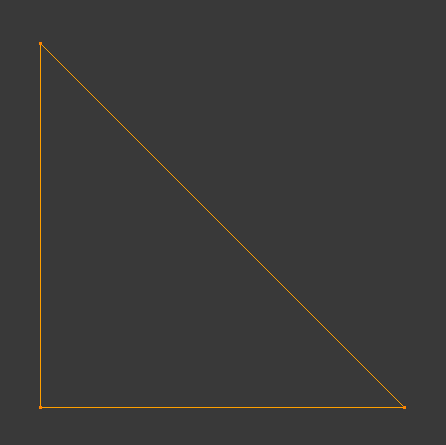
\includegraphics[height=\twosubht]{tex/img/ch03/Basics02_Edges.png}
    }\quad
    \subcaptionbox{\label{fig:3d-face}}{%
        
\includegraphics[height=\twosubht]{tex/img/ch03/Basics03_Faces.png}
    }\quad
    \subcaptionbox{\label{fig:3d-mesh}}{%
        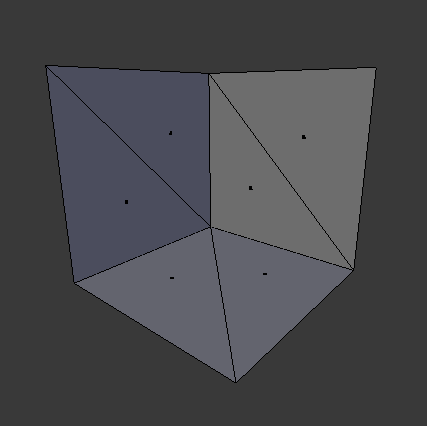
\includegraphics[height=\twosubht]{tex/img/ch03/Basics04_Meshes.png}
    }
    \caption{Construction of a mesh}
    \label{fig:3d-mesh-construction}
\end{figure}

\subsubsection{Materials}
\label{ch03-materials}
\emph{Materials} describe how faces of meshes shall be rendered. They can define properties that are either dependent or independent of the location or size of a surface. Properties that are independent of the location and size of surfaces are often limited to primitive simple features such as color and reflectance.\\
In order to enable more powerful effects, materials need to be able to map each point on a surface of a mesh to a texture coordinate. This process is called UV mapping and it provides a way to "wrap" textures around meshes by defining a 2D coordinate on a texture (using $u$ and $v$ values for width and height in an interval of $[0, 1]$) for each vertex of a mesh \cite{BlenderUVEditor}. Once this map exists, materials can use \emph{texture mapping} to add various effects to a mesh's surface, including:
\begin{description}
    \item[Texture] A \emph{texture} is an image that is wrapped around a mesh so its surfaces show parts of it. They can be used to add great visual detail to meshes that would not be feasible to implement with geometry alone.
    \item[Normal Map] \emph{Normal maps} add geometric visual detail to rendered surfaces by lighting bumps that are not present in the mesh \cite{UnityDocNormalmap}.  This information is calculated from the normals of faces of high-resolution meshes and can then be mapped to low-resolution meshes \cite{Cohen:1998:AS:280814.280832}\cite{745285}. They effectively allow to preserve the visual level of detail of high-resolution meshes while low-resolution meshes are used to save resources in the rendering process.
    \item[Height Map] \emph{Height maps} are similar to normal maps in that they add visual detail geometric visual to surfaces that are not present in the mesh. However they  manipulate the visible area of the surface texture so that individual parts of the surface occlude others and thus give an impression of depth to the surface.
    \item[Specular Map] \emph{Specular maps} are used to control the amount of specular reflectivity of individual parts of surfaces \cite{UnityDocSpecularmap}. This effect is often used to imitate metallic surfaces and requires some form of environment map that can be used to reflect parts of the environment on the surface.
\end{description}
Figure \ref{fig:3d-cube-uv-mapping} shows the UV-map of a cube and a texture laid over it. The texture is wrapped around the cube so that each side shows a number contained within the texture.

\begin{center}
%\begin{figure}[t]
%\centering
    \noindent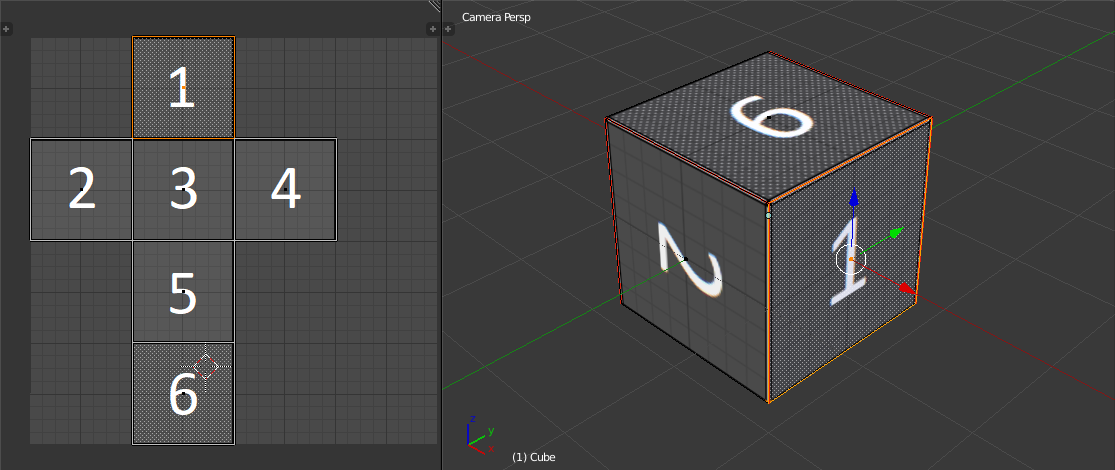
\includegraphics[width=12cm]{tex/img/ch03/CubeUVMapping.png}
    \captionof{figure}[UV-map of a cube]{UV-map of a cube on top of a texture}
    \label{fig:3d-cube-uv-mapping}
%\end{figure}
\end{center}

\subsection{Rendering}
The process of creating images of 3D models or scenes is called \emph{Rendering}. It draws objects contained in scenes from the viewpoint of a virtual camera to a 2D plane and takes materials and lighting information into account. There are two categories of renderers: \emph{offline renderers} usually strive for realistic visual output and use expensive techniques to create images, such as physics-based rendering. The drawbacks of those is that the time they require to render scenes is directly dependent on the scene's complexity. \emph{Online renderers} run in real-time to produce images in quick succession.\\
If these images are generated and shown just quickly enough, movements in the scene appear continuous: in studies, the majority of participants could distinguish modulated light (such as displays) at rates of $50-90 Hz$, however other studies found that this number may be as high as $500 Hz$ \cite{Davis2015}. While there is a scientific disagreement about the rate of images that humans are able to perceive, process and distinguish, the industry introduced standards for electronic displays. Modern displays present images at $60-144 Hz$.\\
The following sections will show two technologies widely used in offline and online renderers.

\subsubsection{Raytracing}
A widely used technology used in offline renderers is \emph{raytracing}. To a certain extend, it imitates real cameras in that for each pixel in the image that is to be rendered, it sends rays from a virtual camera to objects in the scene to calculate the color at the point where it hit an object, considering the material of the surface that was hit. Reflective properties of materials are taken into account by sending rays from the point an object was hit at. Noise and strong contrasts between pixels in the image can be countered by casting multiple rays per pixel and averaging the resulting color.\\
Raytracing is used in software like \emph{Blender} that aims to produce physically correct output.

\subsubsection{Rasterization} Modern games use \emph{rasterization} to render scenes to the screen. This approach processes 3D objects through various stages that differ in their exact implementation but share the same concepts. First, geometry is processed by a \emph{vertex shader} that transforms all vertices of the geometry to screen space (using the transformations shown in \ref{ch03-transforms}). This shader may manipulate properties like color of vertices but it can not create new geometry. The geometry is further passed to a \emph{geometry shader} which, contrary to vertex shaders, may add to the geometry to add detail to it. For instance, it may make use of technologies like tessellation which sub-divides geometry into further triangles to round the silhouette of geometry. The resulting geometry is broken down into \emph{fragments} by discarding vertices that are not visible in the image because they are either not in the field-of-view of the camera (\emph{clipping}) or are not facing the camera (\emph{culling}).
Then the geometry is rasterized: polygons are translated to individual pixels in the \emph{frame buffer}. By performing a so called \emph{depth test} for each pixel, only the geometry that is nearest to the camera will be drawn for an individual pixel.
Lastly, resulting the pixels are passed through a \emph{pixel shader} that may implement various effects of texture maps described in \ref{ch03-materials} such as normal maps and specular maps. They may also manipulate the \emph{z-buffer} that is used to store depth information. When at later stages textures are passed to pixel shaders, they may manipulate the textures by applying two-dimensional effects like blur.\\
\emph{Post-processing} is often done in vertex and pixel shaders and allows to apply effects to the scene that require information about the entire image, such as \emph{anti-aliasing} (used to smooth out hard edges), \emph{bloom} (glow of light seen in real cameras) and blur (e.g. \emph{motion blur} and blur caused by depth in images that is out of focus, \emph{depth of field}).
\clearpage

% //////////////////////////////////////////////////
\section{Game Engines}
Game engines are software environments that provide a set of components that allows to create and run video games. They feature a \emph{rendering} and \emph{audio engine} used for audio and visual output and a \emph{physics engine} to simulate aspects of physics such as gravity and collision. Most feature a so called \emph{game loop} that orchestrates these engines and processes a game's logic (shown in Figure \ref{fig:game-loop}). One cycle of this loop is commonly referred to as a \emph{frame}. Depending on the implementation of the game loop, a game may enter an idle state after rendering to limit the amount of \ac{FPS} or update the scene multiple times per frame at times when updates are required in rapid succession. It may also skip rendering when rendering takes too long and updates need to be processed (\emph{frame skipping}).

\begin{figure}[t]
    \centering
    \noindent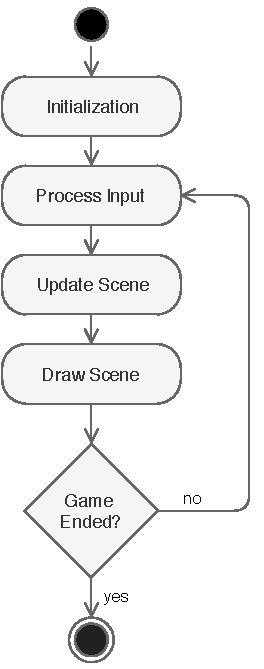
\includegraphics[width=4cm]{tex/img/ch03/GameLoop_04.pdf}
    \captionof{figure}{A simple game loop}
    \label{fig:game-loop}
\end{figure}

\subsection{Development Tools}
The tools used in the development process of games is heavily dependent on the game engine that was used. While some feature a set of command-line tools to pack resources, build folder structures and compile binary executable files, others combine all of these features into one software-suite. \emph{World building} is an essential task in game development and also differs greatly in implementation across game engines: the \emph{Source Engine} (powering \emph{"Half-Life 2"} by \emph{Valve}) requires level designers to use an editor to create scenes (\emph{maps}) and compile them into a proprietary format which is then parsed by the engine at run-time \cite{SourceHammerEditor}. Others, like the \emph{Unreal Engine} (powering \emph{"Life is Strange"} by \emph{Dontnod Entertainment}) and the \emph{Unity Engine} (powering \emph{"Ghost of a Tale"} by \emph{Lionel Gallat}) feature all-in-one editors that combine management of assets and world building \cite{UnrealLevelEditor}\cite{UnityDocsOverview}.

\subsection{Adding Logic to a Game}
While game engines handle sophisticated tasks like rendering and simulating physics on their own, logic is implemented by game developers. There are different ways to add logic to games and this section will focus on two approaches that are widely used.

\subsubsection{Object Oriented Programming}
A traditional approach to enriching entities in scenes with logic is \emph{\ac{OOP}}. In this approach, entities inherit from a base class that holds basic information (e.g. the entity's transform and name) and provides functions used by the engine and other classes that may be overridden (e.g. methods to draw or update the entity). This approach usually works fine for high-level components that manage entities or scenes, however it often involves inheriting multiple classes and when used at a lower level (e.g. on single entities), this results in very complex classes. In scenarios where multiple inheritance is not possible (due to programming language limitations), interfaces may be used. However implementing interfaces multiple times leads to code duplication. Also, behaviours and functionalities are fixed parts of implementations.

\subsubsection{Entity-Component-System}
A common solution to the problems introduced by inheritance in \ac{OOP} is to shift the implementation of interfaces to other classes and make use of composition. \emph{\acp{ECS}} aim to shift the focus from entities as programmable units towards isolated components that represent behaviours. Following the emph{single responsibility principle}, each component is meant to serve and implement a single use. This results in high re-usability of components and reduces code duplication. In \acp{ECS}, entities usually hold a list of components and hence, contrary to \ac{OOP}, entities may have components added to or removed from them at run-time. 